\subsection{High compartmentalization and disparity after gastrulation}
%objective
I estimated the degree of compartmentalization of the Drosophila embryo calculating the relative area of expression of hundreds of genes during development.
My intention was not to focus on individual genes, but to get a global overview of the compartmentalization.

%results
The results showed a non-linear decrease in the mean relative area of expression (an inverted saturation curve), with the major decrease occurring at very early development, from maternal to early gastrula stage (Fig. \ref{fig:Art-I-3measures}).
Practically half of the genes in follows this decrease pattern: 46\% of the genes were characterized as having a non-linear decrease in their relative area.
The results show that the disparity increases non-linearly, again with the major change in the early stages.

It is important to notice that these should not be necessarily the case, as the disparity relates to how different genetically are the different regions of the embryo in different stages, so it could be that between two stages the relative area of expression decreases but not the disparity if the genes are expressed in the same part of the embryo.

%discussion

These results are consistent with the hypothesis that the Drosophila embryo becomes compartmentalized in a progressively more fine-grained manner over developmental time. 
More importantly, they show that this process happens quite early in Drosophila, i.e., around gastrulation.
This is, most genes start being expressed in broad areas of the embryo and over time their expression becomes progressively restricted into smaller and smaller spatial domains.
- Syncitium

%%%%%%%%%%%%%%%%%%%%%%%%%%%%%%%%%%%%%%%%%%%%%%%%%%%%%%%%%%%%%%%%%%%%%%%%%%%%%%%%%%%%% 
\begin{figure}[h]
  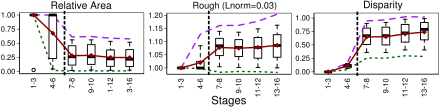
\includegraphics[width=\textwidth]{./Images/Art-I/3_measures.png}
  \centering
  \caption{Distribution plot of the relative area of expression (left), roughness (center) and disparity (right) for all genes in each stage. Diamonds represent the mean, boxes the IQR. Whiskers 10 and 90 percentiles. Dashed line represents the max values and dotted line the min values (mean of the last and first decile, respectively). Stages on the x-axis, vertical dashed line represents gastrulation entry.}
  \label{fig:Art-I-3measures}
\end{figure}
%%%%%%%%%%%%%%%%%%%%%%%%%%%%%%%%%%%%%%%%%%%%%%%%%%%%%%%%%%%%%%%%%%%%%%%%%%%%%%%%%%%%% 

\subsection{The leading role of TFs and GFs}

%objective
I wanted the test the hypothesis that the trascription factors (TFs) and growth factors (GFs) have a a leading role in pattern formation and compartmentalization.
%results 1
The TFs (GO:0003700) and GFs (GO:0008083) showed significantly smaller relative area of expression that the other genes in the blastoderm stage (Fig. \ref{fig:Art-I-3measures}).
	\nomenclature{GF}{Growth Factor}
	\nomenclature{KW}{Kruskal-Wallis test}
	
The TFs are expressed in significantly smaller areas than the rest of the genes in all subsequent stages and the GFs are expressed in smaller areas at the blastoderm stage (stage 4-6) and the extended germ band stages (stage 9-10 and 11-12) (I, Fig.4).

%discussion 1
The TFs results are complementary to the study done by \citet{Hammonds2013}, who made an extensive analysis of TFs expression using the BDGP database, using manual annotation of gene expression based on an anatomical controlled vocabulary and classifying every gene as ubiquitous, patterned, ubiquitous-patterned, or maternal. 
They found that the fraction of TFs expressed in a restricted pattern (assigned to a tissue) was significantly higher, when compared to more than 6000 protein-coding genes, in all the the zygotic stages with the exception of the stage 13-16. The results I show for stages 4-6, 7-8, 9-10 and 11-12 are consistent with Hammonds et al., as the higher proportion of the TF genes showing a restricted or tissue-specific expression pattern would imply that TFs are expressed in smaller areas in the embryo. 
For the 13-16 stage, contrary to these authors, I showed that the TFs are highly compartmentalized. This might indicate a limitation of the annotation method used by Hammonds et al., to capture the high spatial compartmentalization of the TFs in this late stage.

%results & discusion 2
In the blastoderm stage the disparity of the regions based only on the TFs is much greater than the one based on all the genes ((KW pvalue $<0.001$; Fig. \ref{fig:Art-I-3measures}) indicating that these genes account for a large portion of the diversity of gene expression patterns.

In general, the fact that TF genes have lower relative area (i.e., are more compartmentalized) than the rest of the genes, especially in the stage before entering gastrulation, is consistent with the leading role of these genes in driving pattern formation and the resulting compartmentalization of the embryo.

%%%%%%%%%%%%%%%%%%%%%%%%%%%%%%%%%%%%%%%%%%%%%%%%%%%%%%%%%%%%%%%%%%%%%%%%%%%%%%%%%%%%% 
\subsection{Roughness increases non-linearly}
%objective
The roughness measure informs about the overall imbrication or convolution of the shape of a gene expression contour at different spatial scales, relative to a circular shape.
Roughness values equal or close to 1 mean `rounded' patterns (simple) while values greater than 1 mean `convoluted' patterns (complex).
%results
Our results (Fig. \ref{fig:Art-I-3measures}) show that roughness increases in a non-linear way during development, as the major increase is at the transition from the blastoderm to the early gastrula.
The maximal values (mean value of the 10\% of genes that have the higher roughness) increase initially in pre-gastrula stages, reach a stationary phase at mid-embryogenesis and finally increase in the last stages. 
As I mention in the literature review (section X), the maximal values are informative about the overall morphological spatial complexity of the embryo in a given stage.

When comparing roughness at different spatial scales (different Lnorm values; see methods), I found that in the last three stages the roughness values are significantly higher at smaller spatial scales is significantly higher that at the higher spatial scales.(Fig. S2 in article I). 
%discussion
This suggests that complexity may be increasing through all the development but that it would do it at finer and finer spatial scales over time.


%%%%%%%%%%%%%%%%%%%%%%%%%%%%%%%%%%%%%%%%%%%%%%%%%%%%%%%%%%%%%%%%%%%%%%%%%%%%%%%%%%%%% 
\subsection{Main spatio-temporal profiles of gene expression}
%objective
I performed a time series cluster analysis \citep{Ernst2006} using the relative area of expression in order to know which were the most common spatio-temporal profiles (I, Fig. 5).
%results
There were eight different profiles with at least 20 genes assigned, with the profiles with more genes following the global profile of non-linear decrease in the first stages.

Among the rest of profiles, I found both linear increase and decrease profiles and a `mountain-like' profile (initial increase and further decrease with the higher values at stage 7-8)

The linear decrease profile (n=167 genes) was enriched with `mitotic cell cycle' (GO:0000278), `RNA processing' (GO:0006396) and `chromatin modification' (GO:0016568) GOterm genes, highlighting biological processes that first are present in the whole embryo and become more and more restricted in space as development proceeds.
%discussion
The `mitotic cell cycle' term, for example, most likely relates to the fast mitotic cycles in the earliest embryo. During stage 1-3 nine fast and synchronic mitotic divisions take place in the entire embryo, then in stage 4-6 mitotic divisions 10-13 occur more slowly, almost synchronically. The 14th cycle, zygotically controlled, is long and of different durations in the embryo.

In relation to this, \citet{Arbeitman2002} made a temporal co-expression cluster analysis using cDNA microarray data through the life cycle of \textit{D. melanogaster}. They found that most cell cycle genes were expressed at high levels during the first 12 h and only few are expressed at high levels thereafter.
Our analysis is consistent with this, as we found that the profile of linear decrease of relative area of expression (I, Fig. 5A) is enriched with cell cycle genes. 
%Our study is complementary to Arbeitman et al., as we add the spatial dimension to these previously temporally characterized gene expression profiles.

%%%%%%%%%%%%%%%%%%%%%%%%%%%%%%%%%%%%%%%%%%%%%%%%%%%%%%%%%%%%%%%%%%%%%%%%%%%%%%%%%%%%% 
\subsection{Gene synexpression territories in the embryo}
%objective
I used a hierarchical clustering algorithm to produce a dendrogram representing the relative degrees of similarities between embryo regions.
Importantly, I analysed all regions of all the stages at the same time.
After cutting the dendrogram at a certain level and choosing only territories with at least 50 genes expressed with a minimum specificity (see method in I for a detailed description), I ended up with 30 clusters, which I will call from now on `synexpression territories'.
As I wanted to see how the different synexpression territories relate between them, I grouped these (by using another cut-off in the dendrogram) in eight `meta-territories'.

%%%%%%%%%%%%%%%%%%%%%%%%%%%%%%%%%%%%%%%%%%%%%%%%%%%%%%%%%%%%%%%%%%%%%%%%%%%%%%%%%%%%% 
\begin{figure}[h]
  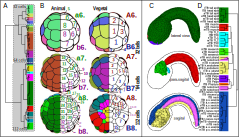
\includegraphics[width=\textwidth]{./Images/Art-I/territories.png}
  \centering
  \caption{Territory analysis on the Drosophila embryo. (A) Dendrogram produced by hierarchical clustering on a similarity matrix (pearson's correlation) of all the embryo regions of the six stages. The red line shows the cut-off to produce 40 territories. (B) Dendrogram with the upper part reconstructed using only territories with at least 50 genes with a minimum specificity of 0.1 (see methods). Areas in gray have less than 50 genes expressed. The coloured boxes show the main branches of the dendrogram. The number indicated inside the boxes represent the stages the territories correspond to (3 is stage 7-8, 4 is stage 9-10, 5 is stage 11-12 and 6 is stage 13-16). The number outside the boxes are the cluster number assigned by the clustering algorithm. (C) Territories in the different embryo stages. Background color refers to which major branch of the dendrogram (in B) each territory is part of. The circles show if the territories are enriched with a GOterm that relates to a specific tissue/germ layer derivative (shown in E). The stage is shown in the lower-left part of each embryo. From stage 7-8, the cluster number (as in B) is indicated inside each territory. (D) Hartenstein's embryo schemes \citep{Hartenstein1993} with their respective stages in the left upper part. (E) Colour code of specific tissue/germ layer derivative used in C.
dataset)}
  \label{fig:Art-I-3measures}
\end{figure}
%%%%%%%%%%%%%%%%%%%%%%%%%%%%%%%%%%%%%%%%%%%%%%%%%%%%%%%%%%%%%%%%%%%%%%%%%%%%%%%%%%%%% 